\section{Discussion and Future Work}
\label{sec:discussion}
In this section, we answer our research questions and discuss our interpretation of this result. We then highlight recommendations to practitioners using QS for collective decision making and highlight future directions for QS.

\subsection{QS effectiveness and its mechanics}
To answer RQ1, which examines how effectively QS captures participant preferences compared to traditional methods, we applied detailed analysis across preference elicitation pairwise results for QS (votes and credit spent), Likert, UQS, and LS. Our analysis demonstrates that QS exhibits superior performance in preference elicitation, though with notable methodological distinctions. For ordinal preference prediction, QS shows a statistically significant but modest advantage over Likert scales. The substantive methodological benefit of QS becomes evident in preference intensity measurement—as the magnitude of preference differentials increases between options, QS maintains high fidelity in capturing these differentials, whereas alternative methodologies demonstrate decreasing accuracy.

Our results also address RQ2, which investigates how the budget constraint and quadratic cost individually and jointly affect preference elicitation quality. Our empirical findings substantiate that both the quadratic cost function and budget constraint constitute essential elements of the QS mechanism. The removal of either component (as implemented in Unlimited QS or Linear Survey) results in diminished performance relative to standard Likert scales, with Linear Survey demonstrating progressively deteriorating accuracy as the allocated budget increases. These results suggest significant caution is warranted when considering simplified variants of QS, as such modifications substantially compromise the mechanism's capacity to accurately reflect underlying preference structures, particularly in contexts where precise measurement of strong preference intensities is crucial.

% insert figure
\begin{figure}[h]
    \centering
    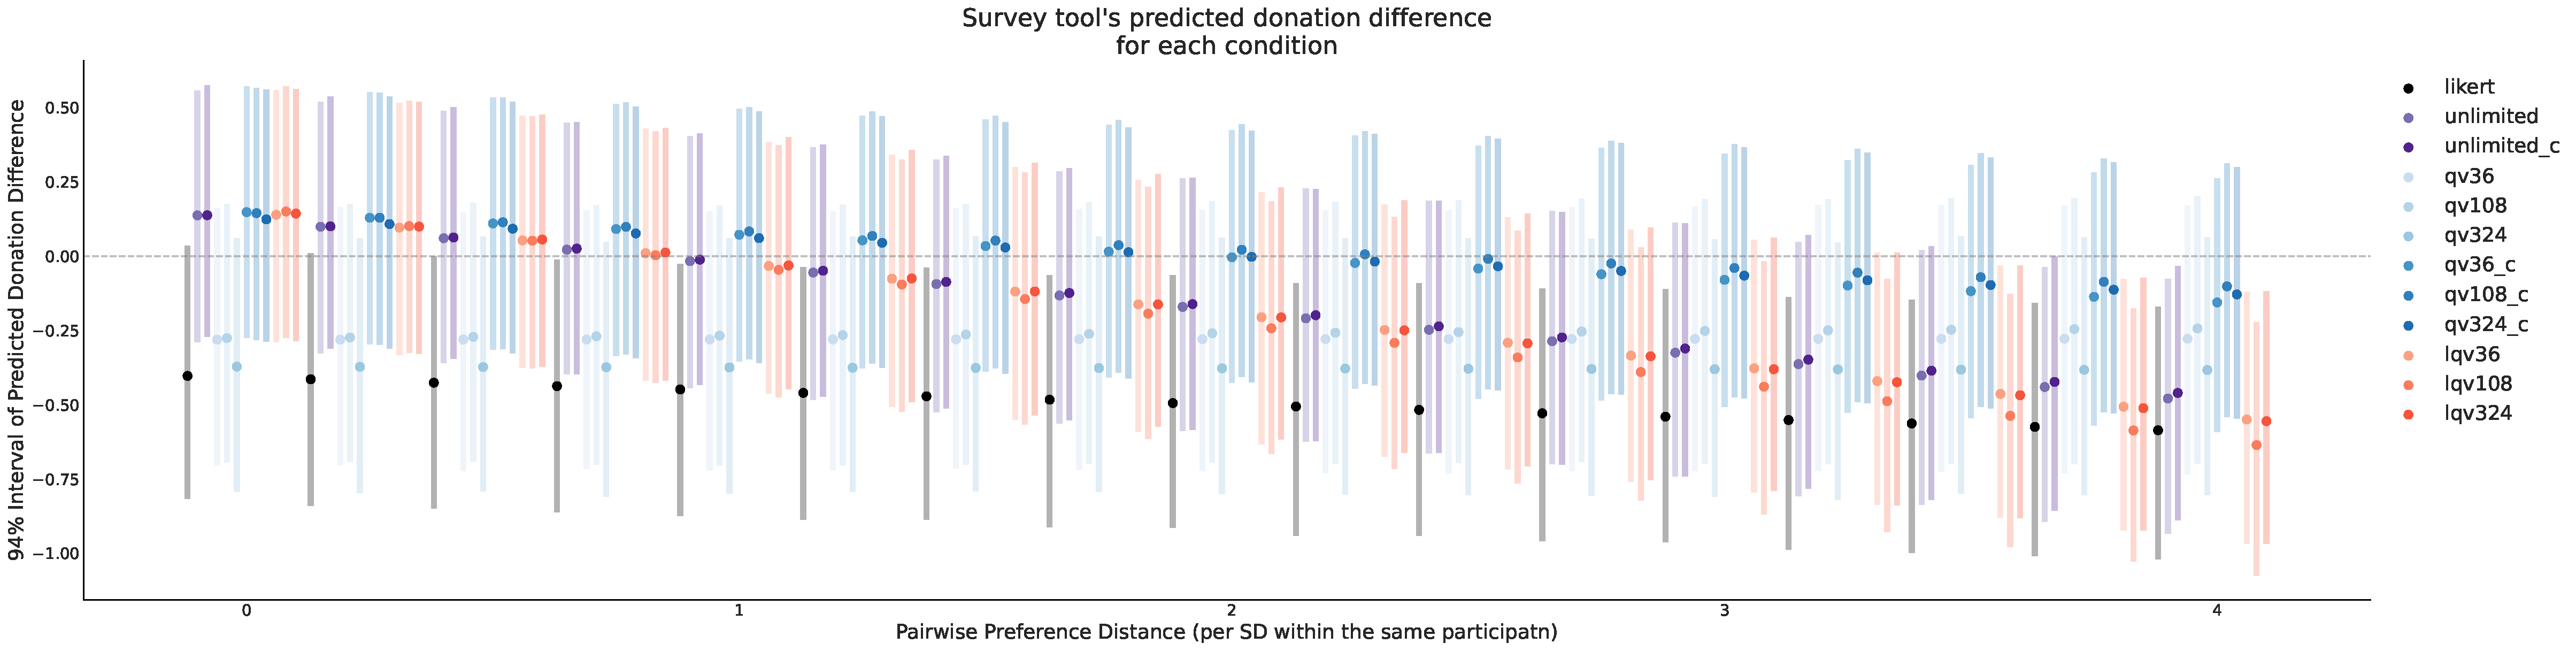
\includegraphics[width=\textwidth]{content/image/Predicted_Donation_Diff_Interval.pdf}
    \caption{Comparison of preference elicitation methods: QS, LS, UQS, and Linear Survey.}
    \label{fig:comparison}
\end{figure}

\subsection{Distortion in survey's `preference units'}
Among options, people have strong preferences between some pairs and less among others.~\Cref{fig:comparison} shows how different survey tools capture the differences 



We interpret the results reflected the diminishing return of additional scales in non QS surveys. The more different one weighs two options, the more underestimation LS and Likert portrays. In intuitive terms, participants should have expressed even stronger preferences to the survey results. The results echo some early constant sum evaluations where experiments show distortions when the individuals allocated more points to specific options~\cite{}.

Because, QS vote costs scaled quadratically, and that participants are indeed weighing the tradeoffs between a provided budget, the budget becomes a good reflection of individual behaviors, as long as the survey designers believes in the assumption that donation is reflective of a person's real world behaviors. In other words, to quantify the actual differences between two options, a practitioner would derive individual's costs to compare it.

\subsection{Votes in QS are designed for aggregation}
The second contribution of this empirical study directly reflects the theoretical goals of Quadratic Voting which the quadratic mechanism aims to prevent tyranny of the majority. If participant's preference intensity aligned well with their donation behaviors, their `perceived' preferences of their response to options are accurate. These credits are then translated as votes as participant's `presented preferences,' which influences the outcome of the group.




% # Relationships Between Linear Voting, Donation Behavior, Budget in Quadratic Surveys, and Quadratic Survey Votes

% ## 1. Linear Voting
% - **Concept**: In linear voting systems, each vote is treated equally, and the cost of each additional vote remains constant.
% - **Outcome**: The difference in vote counts between options directly translates to perceived preference, assuming linear preference increments.
% - **Limitation**: It may not accurately reflect strong intensity differences, as stronger preferences are not weighted differently.

% ## 2. 

% ## 3. Budget in Quadratic Surveys
% - **Concept**: Participants have a limited budget to allocate votes, with costs increasing quadratically.
% - **Outcome**: Forces participants to weigh their choices more carefully, making stronger preferences more costly to express.
% - **Advantage**: Better reflects the strength of preferences as each additional vote requires more effort (cost).
% - **Limitation**: Interpretation of budgets requires understanding the quadratic nature and its impact on expressed preferences.

% ## 4. Quadratic Survey Votes
% - **Concept**: Uses a quadratic cost structure to allocate votes, where each additional vote costs more.
% - **Outcome**: Encapsulates stronger preferences through higher costs, making it harder for majority preferences to dominate without significant effort.
% - **Advantage**: Mitigates tyranny of the majority by making it costlier to exert higher influence.
% - **Interpretation**: The aggregate votes reflect group preferences, but do not linearly correspond to preference strength.

% ## Conclusion
% Understanding these relationships provides a comprehensive view of how different voting mechanisms capture preference intensity.


\section{Limitations and Future work}
\label{sec:limitations}

\paragraph{`True preferences' and survey instruments}
It is important to acknowledge that donation behaviors aims to mirror tangible, monetary contributions that a person would do in real life, which offers real stakes that created such incentive compatible dichotomy. Thus, not all preferences are reflected through monetary means, and external factors might influence donation decisions.

\paragraph{Charities and government roles}
